\section{Inequalities}

\begin{theorem}[Markov's Inequality]
    \label{thm:markov-inequality}%
    Let \(X\) be a non-negative random variable, and \(a > 0\). Then
    \[
        \Prob\para{X \geq a} \leq \frac{\Expt\brac{X}}{a}.
    \]
\end{theorem}

\begin{proof}
    Note the inequality (event)
    \[
        X \geq a \cdot \indicator\para{X \geq a},
    \]
    is always true, since \(X\) is non-negative. Therefore, taking the expectation of both sides, we have
    \[
        \Expt\brac{X} \geq a \cdot \Prob\para{X \geq a}
    \]
    giving as desired.
\end{proof}

\begin{theorem}[Chebyshev's Inequality]
    \label{thm:chebyshev-inequality}%
    Let \(X\) be a random variable with \(\Expt\brac{X} < \infty\). Then for all \(a > 0\), we have
    \[
        \Prob\para{\abs{X - \Expt\brac{X}} \geq a} \leq \frac{\Var\para{X}}{a^2}.
    \]
\end{theorem}

\begin{proof}
    Take \(Y = \para{X - \Expt\brac{X}}^2\) and \(a' = a^2\). Applying Markov's inequality, we have
    \begin{align*}
        \Prob\para{\abs{X - \Expt\brac{X}} > a} &= \Prob\para{\abs{X - \Expt\brac{X}}^2 \geq a^2} \\
        &\leq \frac{\Expt\brac{\para{X - \Expt\brac{X}}^2}}{a^2} \\
        &= \frac{\Var\para{X}}{a^2}.
    \end{align*}
\end{proof}

\begin{theorem}[Cauchy--Schwartz Inequality]
    \label{thm:cauchy-schwartz-inequality}%
    Let \(X\) and \(Y\) be two random variables. Then
    \[
        \Expt\brac{\abs{XY}} \leq \sqrt{\Expt\brac{X^2} \cdot \Expt\brac{Y^2}}
    \]
\end{theorem}

\begin{proof}
    Suppose \(\Expt\brac{X^2} < \infty\) and \(\Expt\brac{Y^2} < \infty\) (otherwise we are done).

    We have
    \[
        \abs{XY} \leq \frac{1}{2} \para{X^2 + Y^2}
    \]
    and hence
    \[
        \Expt\brac{\abs{XY}} < \infty.
    \]

    We assume \(\Expt\brac{X^2} > 0\) and \(\Expt\brac{Y^2} > 0\), otherwise this is trivial. Without loss of generality, also assume \(X, Y \geq 0\) (since we could just take the absolute value of them if they weren't).

    Let \(t \in \RR\), and consider \(\para{X - tY}^2 \geq 0\). Then we have
    \[
        \Expt\brac{\para{X - tY}^2} \geq 0
    \]
    and hence,
    \[
        \Expt\brac{X^2} - 2t \Expt\brac{XY} + t^2 \Expt\brac{Y^2} \geq 0.
    \]

    Taking the derivative of the left-hand side \(f\para{t}\), we have
    \[
        f'\para{t} = -2 \Expt\brac{XY} + 2t \Expt\brac{Y^2}
    \]
    which shows that the minimum is taken at
    \[
        t_0 = \frac{\Expt\brac{XY}}{\Expt\brac{Y^2}}.
    \]

    Hence,
    \[
        \min f\para{t} = f\para{t_0} \geq 0,
    \]
    and hence
    \[
        \Expt\brac{X^2} - 2 \cdot \frac{\para{\Expt\brac{XY}}^2}{\Expt\brac{Y^2}} + \frac{\para{\Expt\brac{XY}}^2}{\Expt\brac{Y^2}} \geq 0.
    \]

    Hence,
    \[
        \para{\Expt\brac{XY}}^2 \leq \Expt\brac{X^2} \cdot \Expt\brac{Y^2}.
    \]
\end{proof}

We now investigate the cases of equality in Cauchy--Schwartz.

We want that
\[
    \Expt\brac{XY} = \sqrt{\Expt\brac{X^2} \cdot \Expt\brac{Y^2}}.
\]

Hence, in particular, we must have that \(f\para{t_0} = 0\). This means
\[
    \Expt\brac{\para{X - t_0 Y}^2} = 0
\]
and hence
\[
    \Prob\para{X - t_0 Y = 0} = 1.
\]

This means that \(\Prob\para{X = t_0 Y}\) and this means \(X\) is a multiple of \(Y\).

\begin{definition}[Convex Function]
    \label{def:convex-fn}%
    A function \(\functiondomain{f}{\RR}{\RR}\) is called \emph{convex}, if for all \(x, y \in \RR\) and \(t \in \ccintv{0}{1}\), we have
    \[
        f\para{tx + \para{1 - t} y} \leq t f\para{x} + \para{1 - t} f\para{y}.
    \]
\end{definition}

\begin{figure}[ht!]
    \centering
    \begin{tikzpicture}
        \begin{axis}[
            axis lines = middle,
            xlabel = {\(x\)},
            ylabel = {\(f\para{x}\)},
            xmin = 0, xmax = 6,
            ymin = 0, ymax = 6,
            samples = 100,
            domain = 0.5:5.5,
            xtick = {2, 3, 5},
            xticklabels = {\(x\), \(tx+\para{1-t}y\), \(y\)},
            ytick = \empty
        ]

            \addplot[no marks] {0.5*(x-3)^2 + 1};
            \node[above left] at (axis cs:5.5,4.125) {\(f\)};

            \addplot[only marks, mark=*, mark size=1pt]
                coordinates {(2, 1.5) (5, 3)};

            \node[below left] at (axis cs:2, 1.5) {\(\para{x, f\para{x}}\)};
            \node[above left] at (axis cs:5, 3) {\(\para{y, f\para{y}}\)};

            \addplot[dashed] coordinates {(2, 1.5) (5, 3)};
            \addplot[only marks, mark=*, mark size=1pt]
                coordinates {(3, 2) (3, 1)};
            \node[above left] at (axis cs:3, 2) {\(t f\para{x} + \para{1 - t} f\para{y}\)};
            \node[below right] at (axis cs:3, 1) {\(f\para{tx + \para{1 - t} y}\)};

            \addplot[dotted] coordinates {(3, 0) (3, 2)};

        \end{axis}
    \end{tikzpicture}

    \caption{Convex Function}
    \label{fig:convex-fn}
\end{figure}

The definition is illustrated in \autoref{fig:convex-fn}.

\begin{theorem}[Jensen's Inequality]
    \label{thm:jensen}%
    Let \(X\) be a random variable, and \(\functiondomain{f}{\RR}{\RR}\) be a convex function. Then
    \[
        \Expt\brac{f\para{X}} \geq f\para{\Expt\brac{X}}.
    \]
\end{theorem}

\begin{figure}[ht!]
    \centering
    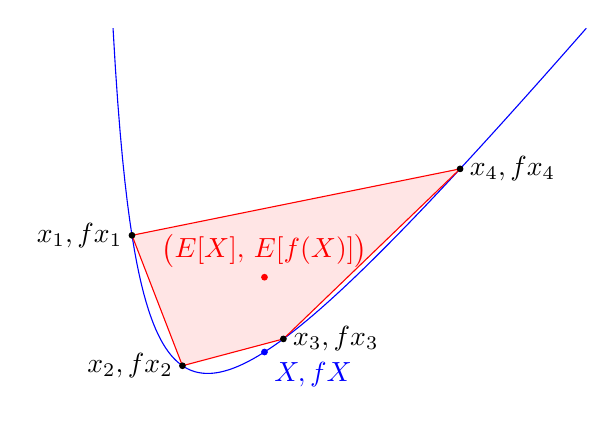
\begin{tikzpicture}
        \begin{axis}[
            axis lines = none,
            xmin = -2, xmax = 4.5,
            ymin = 0, ymax = 4.5,
            samples = 200,
            domain = 0.25:4,
            width = 12cm
        ]

        \addplot[no marks, blue]{1 / x + x};

        \pgfmathsetmacro{\xa}{0.4}
        \pgfmathsetmacro{\xb}{0.8}
        \pgfmathsetmacro{\xc}{1.6}
        \pgfmathsetmacro{\xd}{3}
        \pgfmathsetmacro{\xe}{(\xa + \xb + \xc + \xd) / 4}

        \pgfmathsetmacro{\fa}{1 / \xa + \xa}
        \pgfmathsetmacro{\fb}{1 / \xb + \xb}
        \pgfmathsetmacro{\fc}{1 / \xc + \xc}
        \pgfmathsetmacro{\fd}{1 / \xd + \xd}
        \pgfmathsetmacro{\fe}{1 / \xe + \xe}

        \pgfmathsetmacro{\ef}{(\fa + \fb + \fc + \fd) / 4}

        \addplot[only marks, mark=*, mark size=1pt]
                coordinates {(\xa, \fa) (\xb, \fb) (\xc, \fc) (\xd, \fd)};

        \node[left] at (axis cs:\xa, \fa) {\(\para{x_1, f\para{x_1}}\)};
        \node[left] at (axis cs:\xb, \fb) {\(\para{x_2, f\para{x_2}}\)};
        \node[right] at (axis cs:\xc, \fc) {\(\para{x_3, f\para{x_3}}\)};
        \node[right] at (axis cs:\xd, \fd) {\(\para{x_4, f\para{x_4}}\)};

        \addplot[
            fill=red!10,
            draw=red
        ]
        coordinates {
            (\xa, \fa)
            (\xb, \fb)
            (\xc, \fc)
            (\xd, \fd)
            (\xa, \fa)
        };

        \addplot[only marks, mark=*, mark size=1pt, blue]
            coordinates {(\xe,\fe)};
        \node[blue, below right] at (axis cs:\xe, \fe) {\(\para{\Expt\brac{X}, f\para{\Expt\brac{X}}}\)};

        % (E[X], E[f(X)]) point
        \addplot[only marks, mark=*, mark size=1pt, red]
            coordinates {(\xe,\ef)};

        \node[red, above] at (axis cs:\xe,\ef)
            {$\bigl(\mathbb E[X],\,\mathbb E[f(X)]\bigr)$};
        \end{axis}
    \end{tikzpicture}

    \caption{Jensen's Inequality}
    \label{fig:jensen-inequality}
\end{figure}

A trick to remembering the direction of the inequality is that since
\[
    \Var\para{X} = \Expt\brac{\para{X - \Expt\brac{X}}^2} \geq 0
\]
and also
\[
    \Var\para{X} = \Expt\brac{X^2} - \Expt\brac{X}^2,
\]
and note \(f\para{x} = x^2\) is convex and
\[
    \Expt\brac{X^2} \geq \para{\Expt\brac{X}}^2.
\]

To visualise \autoref{thm:jensen} (Jensen's Inequality), \autoref{fig:jensen-inequality} considers a uniform distribution over \(\brce{x_1, x_2, x_3, x_4}\), and the centre of the quadrilateral is marked red, with \(y\)-coordinate \(\Expt\brac{f\para{X}}\), while \(f\para{\Expt\brac{X}}\) is marked as the blue dot on the curve.

We first produce useful lemmas for the proof.

\begin{lemma}[Convex Function lies above Tangents]
    \label{lem:convex-fn-tangents}%
    A convex function \(\functiondomain{f}{\RR}{\RR}\) is the supremum of all the lines lying below it. In other words,
    \[
        \forall m \in \RR, \exists a, b \in \RR: f\para{m} = am + b \land \forall x \in \RR: f\para{x} \geq ax + b.
    \]
\end{lemma}

\begin{figure}[ht!]
    \centering
    \begin{tikzpicture}
        \begin{axis}[
            axis lines = middle,
            xlabel = {\(x\)},
            ylabel = {\(f(x)\)},
            xmin = -1, xmax = 5,
            ymin = -2, ymax = 9,
            xtick = \empty,
            ytick = \empty,
            domain = 0:4,
            samples = 100,
            width = 10cm
        ]

            \addplot[no marks, thick, blue] {0.5*x^2};

            \addplot[only marks, mark=*, mark size = 1pt] coordinates {(1, 0.5) (2, 2) (3, 4.5)};

            \addplot[domain=0.25:4.5] {1 * (x - 1) + 0.5};
            \addplot[domain=0.4:4.2] {2 * (x - 2) + 2};
            \addplot[domain=0.5:4.1] {3 * (x - 3) + 4.5};
        \end{axis}
    \end{tikzpicture}

    \caption{Convex Function and its Tangents}
    \label{fig:convex-fn-tangents}
\end{figure}

\autoref{fig:convex-fn-tangents} visualises this.

\begin{proof}
    Let \(m \in \RR\) and \(x < m < y\). Then
    \[
        m = tx + \para{1 - t}y
    \]
    for some \(t \in \oointv{0}{1}\). This gives
    \[
        t\para{m - x} = \para{1 - t} \para{y - m}.
    \]

    By convexity,
    \[
        f\para{m} = f\para{tx + \para{1 - t} y} \leq t f\para{x} + \para{1 - t} f\para{y}
    \]
    and hence
    \[
        t\para{f\para{m} - f\para{x}} \leq \para{1 - t} \para{f\para{y} - f\para{m}}.
    \]

    Hence,
    \[
        \frac{f\para{m} - f\para{x}}{m - x} \leq \frac{f\para{y} - f\para{m}}{y - m}.
    \]

    Let
    \[
        a = \sup_{x < m} \frac{f\para{m} - f\para{x}}{m - x}.
    \]

    Then, from the previous inequality on the gradients,
    \[
        \frac{f\para{m} - f\para{x}}{m - x} \leq a \leq \frac{f\para{y} - f\para{m}}{y - m}.
    \]

    So this gives that
    \[
        f\para{z} \geq a\para{z - m} + f\para{m},
    \]
    for all \(z \in \RR\), with the equal sign taking place if \(z = m\).
\end{proof}

Now we use \autoref{lem:convex-fn-tangents} to prove \autoref{thm:jensen} (Jensen's Inequality).

\begin{proof}[of \autoref{thm:jensen} (Jensen's Inequality)]
    Let \(m = \Expt\brac{X}\). By the claim, there is some \(a, b \in \RR\), such that
    \[
        f\para{m} = am + b
    \]
    and
    \[
        f\para{x} \geq ax + b
    \]
    for all \(x\). Then, we have
    \[
        f\para{X} \geq aX + b.
    \]

    Taking expectations on both sides, we get
    \[
        \Expt\brac{f\para{X}} \geq a \Expt\brac{X} + b = am + b = f\para{m} = f\para{\Expt\brac{X}}.
    \]
\end{proof}

Combining both \autoref{lem:convex-fn-tangents}, we can produce a proof as follows.

\begin{proof}[of \autoref{thm:jensen} (Jensen's Inequality), combining \autoref{lem:convex-fn-tangents}]
    Let \(m = \Expt\brac{X}\). For any \(x < m < y\), let \(t \in \ccintv{0}{1}\) be such that
    \[
        m = tx + \para{1 - t} y.
    \]

    Then,
    \[
        t \para{m - x} = \para{1 - t} \para{y - m}. \eqno{(\dagger)}
    \]

    By convexity condition,
    \[
        f \para{m} \leq t x + \para{1 - t} f\para{y},
    \]
    so
    \[
        t \para{f\para{m} - f\para{x}} \leq \para{1 - t} \para{f\para{y} - f\para{m}}. \eqno{(\ddagger)}
    \]

    Dividing \((\ddagger)\) by \((\dagger)\) (since it is positive), we have for all \(x < m < y\), that
    \[
        \frac{f\para{m} - f\para{x}}{m - x} \leq \frac{f\para{y} - f\para{m}}{y - m}.
    \]

    Define
    \[
        a = \sup_{x < m} \frac{f\para{m} - f\para{x}}{m - x},
    \]
    then we have for all \(x < m < y\), that
    \[
        \frac{f\para{m} - f\para{x}}{m - x} \leq a \leq \frac{f\para{y} - f\para{m}}{y - m},
    \]
    so for all \(z \in \RR\) (by dealing with cases \(z < x\) and \(z > y\) using the inequality above)
    \[
        f\para{z} \geq f\para{m} + a \para{x - m}.
    \]

    Therefore,
    \[
        f\para{X} \geq f\para{\Expt\brac{X}} + a \para{x - \Expt\brac{X}},
    \]  
    and taking expectations on both sides, we have
    \[
        \Expt\brac{f\para{X}} \geq f\para{\Expt\brac{X}} + a \para{\Expt\brac{X} - \Expt\brac{X}} = f\para{\Expt\brac{X}}
    \]
    as desired.
\end{proof}

Similar to when we study Cauchy--Schwartz back then, we study the cases of equality.

Let \(\functiondomain{f}{\RR}{\RR}\) be convex, and with the extra property that for \(m = \Expt\brac{X}\), there is some \(a, b \in \RR\), such that
\[
    f\para{m} = am + b \land \forall x \in \RR \setminus \brce{m}: f\para{x} > ax + b,
\]
i.e. let \(f\) be strictly convex at \(m\). Note that 
\[
    f\para{X} - \para{aX + b} \geq 0.
\]

Taking expectation on both sides, we have
\[
    \Expt\brac{f\para{X}} \geq a \Expt\brac{X} + b = am + b = f\para{m} = f\para{\Expt\brac{X}}.
\]

We want that \(\Expt\brac{f\para{X}} = f\para{\Expt\brac{X}}\), so this forces
\[
    \Expt\brac{f\para{X} - \para{aX + b}} = 0
\]
which implies that
\[
    \Prob\para{f\para{X} = aX + b} = 1.
\]

But this now forces \(X = m\), so \(\Prob\para{X = m} = 1\).

There is a nice result due to Jensen's Inequality.

\begin{theorem}[AM--GM Inequality]
    \label{thm:am-gm}
    Let \(f\) be a convex function. Then we have for all \(x_1, \ldots, x_n \in \RR\), we have
    \[
        \frac{1}{n} \sum_{k = 1}^{n} f\para{x_k} \geq f\para{\frac{\sum_{k = 1}^{n} x_k}{n}}.
    \]
\end{theorem}

\begin{proof}
    We take \(X\) to be a random variable, with \(X \sim \Uniform \brce{x_1, x_2, \ldots, x_n}\), with \(\Prob\para{X = x_i} = \frac{1}{n}\) for \(i = 1, 2, \ldots, n\).

    Hence,
    \[
        \frac{1}{n} \sum_{k = 1}^{n} f\para{x_k} = \Expt\brac{f\para{X}} = \sum_{x \in \RR} f\para{x} \Prob\para{X = x}.
    \]

    By \autoref{thm:jensen} (Jensen's Inequality), we have
    \[
        \Expt\brac{f\para{X}} \geq f\para{\Expt\brac{X}} = f\para{\frac{\sum_{k = 1}^{n} x_k}{n}}.
    \]
\end{proof}

\begin{remark}
    The more commonly seen AM--GM inequality is a corollary of this. Let \(f\para{x} = - \log x\), for \(x > 0\). Take \(x_1, \ldots, x_n > 0\), we have
    \[
        - \frac{1}{n} \sum_{k = 1}^{n} \log x_k \geq - \log \para{\frac{\sum_{k = 1}^{n} x_k}{n}}.
    \]

    Exponentiating both sides, we get
    \[
        \para{\prod_{k = 1}^{n} x_k}^{\frac{1}{n}} \leq \frac{1}{n} \sum_{k = 1}^{n} x_k.
    \]
\end{remark}